%----------------------------------------------------------------------------------------
%   PACKAGES AND DOCUMENT CONFIGURATIONS
%----------------------------------------------------------------------------------------

\documentclass[12pt]{article}
\usepackage[english]{babel}
\usepackage[utf8]{inputenc}
\usepackage{float}

\usepackage{graphicx,epstopdf}   %for embedding images and for conveting eps to pdf
\usepackage{subfig}              %for sub images
\usepackage[margin=1in,includefoot]{geometry}	%changes the margins of report to 1 in
\usepackage{lscape}

\usepackage{rotating}   %used for rotating figures
\usepackage[automake,nonumberlist]{glossaries}    %To use glossary
\usepackage{varwidth}
\usepackage{multicol}   %for making columns
\usepackage{amsmath}
\usepackage{appendix}
\usepackage{pdfpages}
\usepackage{empheq}

\usepackage[framed, numbered]{matlab-prettifier}    %to import matlab code

%----------------------------------------------------------------------------------------
%   Acronym/Glossary
%----------------------------------------------------------------------------------------
\makeglossaries
\loadglsentries{glossary}

%----------------------------------------------------------------------------------------
%   Document Start
%----------------------------------------------------------------------------------------

\begin{document}

\begin{titlepage}

\newcommand{\HRule}{\rule{\linewidth}{0.5mm}} % Defines a new command for the horizontal lines, change thickness here

\center % Center everything on the page
 
%----------------------------------------------------------------------------------------
%   HEADING SECTIONS
%----------------------------------------------------------------------------------------

\textsc{\LARGE MSE 480 Manufacturing Systems}\\[1.5cm] % Org Name
\textsc{\Large }\\[0.5cm] % course name
\textsc{\large }\\[0.5cm] % course title

%----------------------------------------------------------------------------------------
%   TITLE SECTION
%----------------------------------------------------------------------------------------

\HRule \\[0.4cm]
{ \huge \bfseries Lab 2: Robotics - Prelab}\\[0.4cm] % Title of report
\HRule \\[1.5cm]
 
%----------------------------------------------------------------------------------------
%   AUTHOR SECTION
%----------------------------------------------------------------------------------------

\begin{minipage}{0.4\textwidth}
    \begin{flushleft} \large
        \emph{Authors:}\\
        Parshant \textsc{Bombhi}\\
        Klark \textsc{Li}
    \end{flushleft}
\end{minipage}
\hfill
\begin{minipage}{0.4\textwidth}
    \begin{flushright} \large
        \emph{Student ID:} \\
        301255126\\
        301276715
    \end{flushright}
\end{minipage}
\vspace{10mm}
%----------------------------------------------------------------------------------------
%   DATE SECTION
%----------------------------------------------------------------------------------------

{\large \today}\\[2cm] % Date, change the \today to a set date if you want to be precise

%----------------------------------------------------------------------------------------
%   LOGO SECTION
%----------------------------------------------------------------------------------------


\includegraphics[scale=2.0]{MSE-Logo.jpg}\\[1cm] %logo
%----------------------------------------------------------------------------------------

\vfill % Fill the rest of the page with whitespace

\end{titlepage}

%----------------------------------------------------------------------------------------
%   Table of Contents/Table of Figures
%----------------------------------------------------------------------------------------
\pagenumbering{roman} %sets numbering of page to roman
\tableofcontents	%makes table of contents
\addcontentsline{toc}{section}{\numberline{}Table Of Contents}	%adds TOC to TOC

\listoffigures
\addcontentsline{toc}{section}{\numberline{}List of Figures}	%adds list of figures to table of contents

 \listoftables
 \addcontentsline{toc}{section}{\numberline{}List of Tables}

\lstlistoflistings
\addcontentsline{toc}{section}{\numberline{}Listings}

% \printglossary
% \addcontentsline{toc}{section}{\numberline{}Glossary}	%adds glossary to table of contents
\pagebreak
%----------------------------------------------------------------------------------------
%   Main Body
%----------------------------------------------------------------------------------------
\setcounter{page}{1}	%resets the page numbering
\pagenumbering{arabic}	%sets numbering of page to arabic
\setlength{\parskip}{1em}

\section{Introduction}
In this prelab we were to find a forward kinematics solution to a AL5D robot. We used the coordinate frames assigned in figure \ref{fig:frames} and created the homogeneous transformation matrix $A_{i}$ for each link. Then we created a transformation matrix $T_{0t}$ to find the end effector rotation and orientation based on the rotation of the joints as given by the cases provided.

\begin{figure}[H]
    \centering
    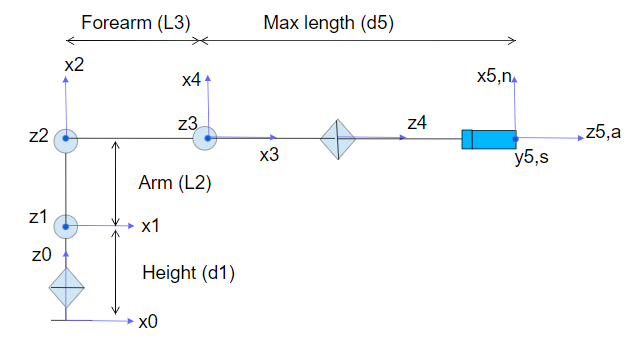
\includegraphics[width=0.8\textwidth]{frames.png}
    \caption{Schematic Diagram of AL5D with Coordinate Frames Assigned}
    \label{fig:frames}
\end{figure}

% Table generated by Excel2LaTeX from sheet 'Sheet1'
\begin{table}[htbp]
  \centering
  \caption{Test Cases}
    \begin{tabular}{|r|rrrrr|}
    \hline
    \multicolumn{1}{|l|}{Case} & \multicolumn{1}{l}{$\theta_1$(deg)} & \multicolumn{1}{l}{$\theta_2$(deg)} & \multicolumn{1}{l}{$\theta_3$(deg)} & \multicolumn{1}{l}{$\theta_4$(deg)} & \multicolumn{1}{l|}{$\theta_5$(deg)} \\
    \hline
    1     & 0     & 0     & 0     & 0     & -90 \\
    2     & 0     & -16.6 & -37.5 & 54.1  & 0 \\
    3     & 33.7  & -8.1  & -23.4 & -58.4 & 33.7 \\
    4     & -33.7 & -8.1  & -23.4 & -58.4 & -33.7 \\
    \hline
    \end{tabular}%
  \label{tab:cases}%
\end{table}%
\pagebreak

\section{Transformation Matrix}
The homogeneous transformation matrix is defined as:
\[
   A_i=\begin{bmatrix}
     c\theta_i & -s\theta_ic\alpha_i & s\theta_is\alpha_i & a_ic\theta_i \\
     s\theta_i & c\theta_ic\alpha_i & -c\theta_is\alpha_1 & a_ic\theta_i \\
     0 & s\alpha_i & c\alpha_i & d_i \\
     0 & 0 & 0 & 1
   \end{bmatrix}
\]
To create the homogeneous transformation matrix we first list out all the D-H parameters the are used in the matrix.
\setlength{\tabcolsep}{12pt}
% Table generated by Excel2LaTeX from sheet 'Sheet1'
\begin{table}[htbp]
  \centering
  \caption{D-H Parameters}
    \begin{tabular}{|l|rrrr|}
    \hline
          & \multicolumn{1}{l}{$\theta$} & \multicolumn{1}{l}{$d$} & \multicolumn{1}{l}{$a$} & \multicolumn{1}{l|}{$\alpha$} \\
    \hline
    $A_{01}$   & $\theta_1$     & $d_1$     & 0     & $\frac{\pi}{2}$ \\
    $A_{12}$   & $\theta_2 + \frac{\pi}{2}$     & 0     & $L_2$     & 0 \\
    $A_{23}$   & $\theta_3 - \frac{\pi}{2}$     & 0     & $L_3$     & 0 \\
    $A_{34}$   & $\theta_4 + \frac{\pi}{2}$     & 0     & 0     & $\frac{\pi}{2}$ \\
    $A_{45}$   & $\theta_5$     & $d_5$     & 0     & 0 \\
    \hline
    \end{tabular}%
\end{table}%

Using these parameters we create the homogeneous transformation matrix and then use them to create a transformation matrix for the system.
\begin{equation}
    T_{0t}=A_{01}A_{12}A_{23}A_{34}A_{45}
\end{equation}
The rotation of the end effector is given by the 3x3 matrix inscribed in the transformation matrix and the orientation is given by the last column.
\[
T_{0t}=\begin{bmatrix}
R&O\\
0&1
\end{bmatrix}
\]
\pagebreak
\section{Results}
By inputting the rotation angles given for each joint we found transformation matrix for each case.\\
\textbf{Case 1:}\\
\[
T_{0t} =
\begin{bmatrix}
         0 & 0 & 1 & 28.576\\
         1 & 0 & 0 & 0\\
         0 & 1 & 0 & 20.789\\
         0 & 0 & 0 & 1
\end{bmatrix}
\]
\textbf{Case 2:}\\
\[
T_{0t} =
\begin{bmatrix}
         0 & 0 & 1 & 25\\
         0 & -1 & 0 & 0\\
         1 & 0 & 0 & 5.0148\\
         0 & 0 & 0 & 1
\end{bmatrix}
\]
\textbf{Case 3:}\\
\[
T_{0t} =
\begin{bmatrix}
         1 & 0 & 0.0015 & 15.0147\\
         0 & -1 & 0.0010 & 10.0136\\
         0.0015 & -0.0010 & -1 & 1.0213\\
         0 & 0 & 0 & 1
\end{bmatrix}
\]
\textbf{Case 4:}\\
\[
T_{0t} =
\begin{bmatrix}
         0.3843 & 0.9232 & 0.0015 & 15.0147\\
         0.9232 & -0.3843 & 0.0010 & 10.0136\\
         0.0015 & 0.0010 & -1 & 1.0213\\
         0 & 0 & 0 & 1
\end{bmatrix}
\]
From the resultant transformation matrix we can find the rotation and orientation of the end effector.

We can further solve for the angle of rotation of the end effector by taking the four quadrant inverse tangent of the rotation matrix. Thus giving us:
% Table generated by Excel2LaTeX from sheet 'Sheet1'
\begin{table}[htbp]
  \centering
  \caption{Final Position and Orientation}
    \begin{tabular}{|l|ll|}
    \hline
          & Position(x,y,z) & Rotation($\theta,\phi,\rho$) \\
    \hline
    Case 1 & (28.5760,0,20.7980) & (90,0,90) \\
    Case 2 & (25,0,5.0148) & (0,-90,180) \\
    Case 3 & (15.0147,10.0136,1.0213) & (-179.94,-0.0832,-4.03E-5) \\
    Case 4 & (15.0147,10.0136,1.0213) & (179.94,-0.0832,67.4) \\
    \hline
    \end{tabular}%
\end{table}%
\pagebreak

\appendix
\section{Matlab Code}
\lstinputlisting[style=Matlab-editor, basicstyle=\mlttfamily\scriptsize, caption={Matlab Code for Transformation Matrix}]{MSE480_Lab2_Prelab.m}
\end{document}
              
            